\documentclass{article}
\usepackage[a4paper, top=3cm, bottom=2.5cm, left=2.5cm, right=2.5cm]{geometry} % Ajuste de márgenes
\usepackage[spanish]{babel}
\usepackage[utf8]{inputenc}
\usepackage{tabularx}
\usepackage{tikz}
\usetikzlibrary{mindmap, shapes, positioning}
\usepackage{titling}
\usepackage{graphicx}
\usepackage{fancyhdr}
\usepackage{amsmath}
\usepackage{amssymb}
\usepackage{multicol}
\usepackage{cancel}
\usepackage{pgfplots}
\usepackage{hyperref}
\pgfplotsset{compat=1.18}
\usepackage{titlesec} % Para personalizar títulos
\usepackage{tocloft}  % Para mejorar el índice
\usepackage{setspace} % Para controlar el espaciado

% Configuración de Fancyhdr para encabezados y pies de página
\pagestyle{fancy}
\fancyhf{}
\fancyhead[L]{
\includegraphics[width=2cm]{assets/logo-utp.png}}
\fancyhead[R]{\textit{Administración y organización de empresas.}}

\fancyfoot[R]{\thepage} % Número de página alineado a la derecha

% Ajustes de espaciado entre párrafos y márgenes superiores
\setlength{\parskip}{1.5em}
\setlength{\parindent}{0pt}
\setlength{\headheight}{17.26935pt} % Altura del encabezado
\addtolength{\topmargin}{-2.26935pt} % Compensar el aumento de la altura del encabezado
\setlength{\textheight}{23cm}  % Ajusta el alto del texto

% Definición de comandos personalizados
\newcommand{\SubItem}[1]{
    {\setlength\itemindent{15pt} \item[-] #1}
}

\pagenumbering{gobble}

% Título del documento con mejor control de espaciado
\title{
  
\includegraphics[width=5cm]{./assets/logo-utp.png} \\
  \vspace{1cm}
  \textbf{Universidad Tecnológica del Perú} \\
  \vspace{2cm}
  \textbf{Diagnóstico de la Gestión Comercial en la Empresa Nvidia.} \\
  \vspace{1cm}
  \large \textbf{Para el curso de Administración y organización de empresas.}
}

% Ayerbe Balderrama, Juan Carlos 		U19219954 
% Villanueva Ventura Johan James		U24267335 
% Cuya Javier Katerine Carolina			U24261533 
% Huatay Salcedo Luis Elías					U24218809 
% Dante Daniel Lazo Pamucena				U24266885 

\author{
  \begin{tabular}{ll}
    Ayerbe Balderrama, Juan Carlos 	& U19219954 \\
    Cuya Javier, Katerine Carolina & U24261533 \\
    Huatay Salcedo, Luis Elías & U24218809 \\
    Villanueva Ventura Johan James	& U24267335 \\
    Dante Daniel Lazo Pamucena & U24266885
  \end{tabular} \\\\
  \texttt{Sección 43925}
}

% ENVIROMENTS

\newenvironment{indexPre}{}{}
\newenvironment{introduccion}{}{}
\newenvironment{marcoTeorico}{}{}
\newenvironment{problematica}{}{}
\newenvironment{objetivoGeneral}{}{}
\newenvironment{terminosEstadisticos}{}{}
\newenvironment{recoleccionDeInformacion}{}{}
\newenvironment{metodologia}{}{}
\newenvironment{analisisDescriptivo}{}{}

\begin{document}
\maketitle

\begin{center}
  Docente. Mg. Sandra Mariana, Flores Ganoza
\end{center}

\restoregeometry

\pagenumbering{arabic} % Numeración arábiga para el resto del documento
\setcounter{page}{2}   % Iniciar numeración en la página 2

\newpage

\tableofcontents

\newpage

\vspace*{\fill}

\begin{introduccion}
  \section{Introducción}

  Nvidia es una empresa multinacional con sede en Santa Clara, California, que se especializa en el diseño y fabricación de unidades de procesamiento gráfico (GPU) para aplicaciones en gaming, inteligencia artificial, visualización profesional y centros de datos. La empresa ha experimentado un crecimiento significativo en los últimos años, gracias a su enfoque en la innovación y la calidad de sus productos.

  El presente informe tiene como objetivo realizar un diagnóstico de la gestión comercial de la empresa Nvidia, una compañía líder en el mercado de tarjetas gráficas y soluciones de cómputo de alto rendimiento. Para ello, se analizarán aspectos clave de la gestión comercial de la empresa, como su gestión del marketing, ventas, servicio, personal y retención del personal.
    
\end{introduccion}

\vspace*{\fill}

\newpage

\begin{marcoTeorico}
  \section{Marco teórico}

  \subsection{Marketing Mix, las 4 P's}

  Las 4 P's del marketing mix son un conjunto de variables que las empresas pueden controlar para influir en la demanda de sus productos o servicios. Las 4 P's son:
  
  \begin{itemize}
    \item \textbf{Producto:} Se refiere a los bienes o servicios que la empresa ofrece a sus clientes. Nvidia ofrece una amplia gama de productos, desde tarjetas gráficas para gaming hasta soluciones de cómputo de alto rendimiento para centros de datos.
    \item \textbf{Precio:} Se refiere al valor monetario que los clientes están dispuestos a pagar por los productos o servicios de la empresa. Nvidia utiliza una estrategia de precios premium para sus productos de alta gama, basada en su calidad y rendimiento.
    \item \textbf{Plaza:} Se refiere a los canales de distribución que la empresa utiliza para llevar sus productos o servicios al mercado. Nvidia vende sus productos a través de distribuidores autorizados, tiendas en línea y socios comerciales.
    \item \textbf{Promoción:} Se refiere a las estrategias de comunicación que la empresa utiliza para dar a conocer sus productos o servicios y persuadir a los clientes a comprarlos. Nvidia utiliza una combinación de publicidad, relaciones públicas y marketing digital para promocionar sus productos.
  \end{itemize}

  Según Paucar J. (2019), El Marketing Mix es un conjunto de decisiones sobre producto precio, canales de distribución y comunicaciones (o promoción) con las que se despliega la estrategia de marketing. También llamadas las 4 P del marketing por sus siglas en inglés y sus componentes están interrelacionados.

  \begin{flushright}
    \textit{Paucar J. (2019) Evolución de las 4P´s o Marketing Mix.}
  \end{flushright}  

  \subsection{Gestión de Ventas}

  La gestión de ventas es el proceso de planificar, organizar, dirigir y controlar las actividades de ventas de una empresa para alcanzar sus objetivos comerciales. La gestión de ventas implica la identificación de oportunidades de venta, la prospección de clientes, la presentación de propuestas comerciales, el cierre de ventas y el seguimiento postventa.

  Según Rojas Z. (2017). La gestión de ventas es muy importante en el desarrollo, crecimiento y continuidad de
  las empresas de cualquier sector de empresarial, sea comercial, de servicios, industrial,
  etc. El planificar la gestión de ventas y costos es indispensable para establecer las guías
  de acciones necesarias para poder obtener una buena rentabilidad durante el ejercicio
  fiscal.

  \begin{flushright}
    \textit{  Rojas Z. (2017) La Gestión de Ventas y Rentabilidad.}
  \end{flushright}

  \subsection{Gestión del servicio}

  La gestión del servicio es el proceso de planificar, organizar, dirigir y controlar las actividades de servicio al cliente de una empresa para garantizar la satisfacción del cliente y la fidelización. La gestión del servicio implica la atención al cliente, la resolución de problemas, la gestión de reclamos y la mejora continua de la calidad del servicio.

  Según  Piñeiro A. Varela J. Rail A. (2006), Partiendo de la importancia y la valoración que los usuarios otorgan a cada uno de los atributos relevantes de un servicio,es posible obtener una herramienta en los que se incluyan recomendacionespara la gestión de los recursos organizacionales. Sin embargo, esta herramienta ha estado sujeta a controversias desde sus orígenes.

  \begin{flushright}
    \textit{ Piñeiro A. Varela J. Rail A. (2006) El análisis de importancia-valoración aplicado a la gestión de servicios}
  \end{flushright}

  \subsection{Gestión del personal}

    La gestión del personal es el proceso de planificar, organizar, dirigir y controlar las actividades relacionadas con el personal de una empresa para garantizar su eficiencia y productividad. La gestión del personal implica la selección, contratación, capacitación, evaluación y desarrollo del personal, así como la gestión de las relaciones laborales y la prevención de conflictos.

    Según Hernández A. (2006), Un verdadero sistema de provisión de empleos de carrera debe caracterizarse por la consonancia que exista entre el diseño normativo y la aplicación práctica que de él se haga, pues poco será el aporte de 
    un conjunto regulatorio armónico, coherente, ágil y moderno en esta materia si la realidad 
    administrativa no concuerda con tales postulados.

    \begin{flushright}
      \textit{Hernández A. (2006) La provisión de empleos de carrera en Colombia: lineamientos de un nuevo modelo de gestión de personal en el sector público}
    \end{flushright}

\end{marcoTeorico}

\newpage

\begin{objetivoGeneral}
  \section{Objetivo general}

  Realizar un diagnóstico de la gestión comercial de la empresa Nvidia, identificando sus fortalezas y oportunidades de mejora en las áreas de marketing, ventas, servicio, personal y retención del personal.
  
  \subsection{Objetivos específicos}
  
  \begin{enumerate}
    \item Analizar la gestión del marketing de Nvidia, evaluando su estrategia de producto, precio, plaza y promoción.
    \item Evaluar la gestión de ventas de Nvidia, identificando sus procesos de prospección, presentación, cierre y seguimiento de ventas.
    \item Analizar la gestión del servicio al cliente de Nvidia, evaluando su atención al cliente, resolución de problemas y gestión de reclamos.
    \item Evaluar la gestión del personal de Nvidia, identificando sus procesos de selección, contratación, capacitación, evaluación y desarrollo del personal.
    \item Identificar las estrategias de retención del personal de Nvidia, evaluando su clima laboral, beneficios y programas de desarrollo profesional.
  \end{enumerate}
\end{objetivoGeneral}

\newpage

\section{Gestión del marketing}

La estrategia de marketing mix de Nvidia se centra en los cuatro pilares fundamentales: Producto, Precio, Plaza (Distribución) y Promoción. Cada uno de estos componentes juega un papel crucial en el plan de marketing de Nvidia como líder en el mercado de tecnología y en la conformación de su identidad de marca. 

A continuación, se explican cómo NVIDIA, una empresa líder en tecnología y semiconductores, utiliza cada una de estas "P" en su estrategia de marketing: 

\subsection{Producto}

Nvidia se ha establecido como un líder indiscutible en el desarrollo de unidades de procesamiento gráfico (GPU) con los mejores componentes de las tarjetas gráficas, pero su catálogo de productos se extiende mucho más allá. La compañía ha incursionado exitosamente en mercados como la inteligencia artificial (IA), la computación en la nube, la conducción autónoma y la realidad virtual, ofreciendo soluciones de hardware y software innovadoras. La diversificación y la innovación constante en su oferta de productos permiten a Nvidia mantener su relevancia y liderazgo tecnológico.

\begin{itemize}
  \item Centrarse en las soluciones aceleradas de computación y IA.
  \item Las GPU de los juegos, especialmente la serie GeForce RTX 40.
  \item Productos de visualización profesional que ganan tracción.
  \item Soluciones automotrices para la cabina de IA y las plataformas de conducción autónoma.
  \item Diversas aplicaciones en centros de datos, juegos y sectores automotrices.
\end{itemize}

\subsection{Precio}

La estrategia de precios de Nvidia refleja el valor y la calidad premium de sus productos. Con productos que a menudo lideran el mercado en términos de innovación y rendimiento, Nvidia adopta una estrategia de precios que puede considerarse de «precio-premium». Esto se alinea con la percepción de marca y la propuesta de valor que ofrece a sus consumidores, destacando la avanzada tecnología y el rendimiento superior de sus productos.

\begin{itemize}
  \item Estrategia de precios premium para GPU de alto rendimiento.
  \item Precios competitivos en segmentos de juego para capturar la cuota de mercado.
  \item Precios basados en el valor para soluciones de IA que reflejan ROI para empresas.
  \item Actualizaciones periódicas sobre los precios en respuesta a los cambios en el mercado.
  \item Descuentos y paquetes durante los períodos promocionales.
\end{itemize}

\subsection{Plaza}

Nvidia utiliza una estrategia de distribución multicanal para asegurar que sus productos estén ampliamente disponibles para una variedad de consumidores en todo el mundo. Esto incluye la venta directa a través de su sitio web, la distribución a través de minoristas en línea y físicos, y asociaciones con fabricantes de equipos originales (OEMs). Esta amplia red de distribución asegura que los productos de Nvidia sean accesibles para consumidores en diferentes segmentos de mercado, desde entusiastas de los videojuegos hasta profesionales de la industria. No solo es uno de los mejores en la distribución, sino que mejora las de otras industrias con tecnología IA. 

\begin{itemize}
  \item Fuerte presencia en Asia, particularmente China y Taiwán.
  \item Plataformas en línea para productos de consumo, incluida GeForce Now.
\end{itemize}

\subsection{Promoción}

La promoción es donde Nvidia realmente brilla, utilizando una combinación de marketing digital, patrocinios, colaboraciones y eventos para comunicar su marca y productos. La compañía mantiene una presencia activa y comprometida en las redes sociales, aprovecha el marketing de influencers dentro de la comunidad de gaming y tecnología, y participa en eventos y conferencias internacionales para demostrar su liderazgo tecnológico. Campañas publicitarias creativas y colaboraciones con desarrolladores de juegos y aplicaciones resaltan las capacidades de sus productos, mientras que iniciativas como la creación de contenido educativo y demostraciones interactivas fortalecen su posición como líder de pensamiento en la industria tecnológica. 

\begin{itemize}
  \item Estrategias de marketing agresivas para juegos y productos de IA.
  \item Participación en conferencias de la industria y exposiciones tecnológicas.
  \item Involucrar el marketing de contenidos a través de los canales de redes sociales.
  \item Colaboraciones con desarrolladores de juegos para promocionar nuevos títulos.
  \item Uso del marketing de influencia dentro de las comunidades de juego.
  \item Iniciativas educativas que destacan las capacidades de IA y de aprendizaje profundo.
\end{itemize}

% \begin{center}
%   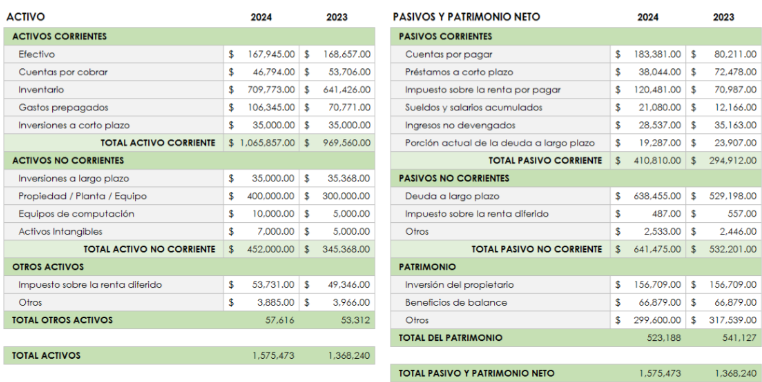
\includegraphics[width=15cm]{./assets/balance.png}
% \end{center}
% \begin{center}
%   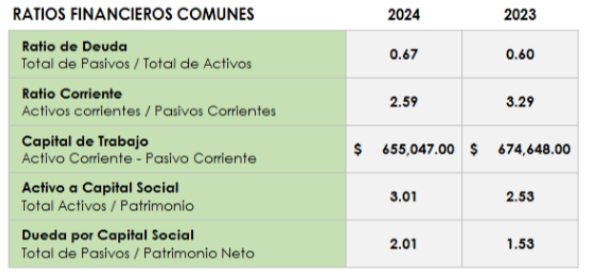
\includegraphics[width=8cm]{./assets/ratios_financieros.png}
% \end{center}

\newpage
\section{Gestión de Ventas}

La gestión de ventas de Nvidia se centra en la identificación de oportunidades de venta, la prospección de clientes, la presentación de propuestas comerciales, el cierre de ventas y el seguimiento postventa. La empresa utiliza un enfoque consultivo para la venta de sus productos y servicios, que se basa en la comprensión de las necesidades y deseos de los clientes y en la presentación de soluciones personalizadas que satisfagan sus requerimientos.

NVIDIA además de la mencionada utiliza diversas estrategias específicas para cerrar ventas, estas estrategias están diseñadas para persuadir a los clientes y garantizar que tomen la decisión de compra. 

Algunas de las estrategias más destacadas son: 

\begin{itemize}
  \item \textbf{Ofrecer Valor Tangible y Diferenciación:} Demostraciones Prácticas: NVIDIA organiza eventos, presentaciones y videos donde muestra el rendimiento real de sus productos, como gráficos avanzados, inteligencia artificial o simulaciones en tiempo real. Esto ayuda a los clientes a visualizar el valor que obtendrán. 

  Comparación con la Competencia: Destaca características únicas, como su tecnología RTX para trazado de rayos y la eficiencia energética de sus chips frente a alternativas del mercado. 

  \item \textbf{Paquetes de Valor Añadido:} Incluye Software Complementario: Ofrecen programas como NVIDIA GeForce Experience o herramientas profesionales como Omniverse sin costo adicional, mejorando el valor del producto. 

  Promociones de Juegos y Servicios: En el segmento de gaming, NVIDIA ofrece juegos gratuitos o descuentos en títulos selectos al comprar sus GPUs, haciendo la oferta más atractiva. 

  \item \textbf{Argumentos de Rentabilidad a Largo Plazo:} En el mercado empresarial, NVIDIA enfatiza el retorno de inversión (ROI). Por ejemplo, en sus GPUs para inteligencia artificial o centros de datos, argumentan que sus soluciones reducen costos operativos debido a su alta eficiencia y rendimiento.  
  En gaming, destacan la durabilidad y soporte continuo, mostrando que sus productos mantienen su relevancia durante años. 

  \item \textbf{Creación de Escasez y Exclusividad:} NVIDIA a menudo utiliza la estrategia de escasez durante lanzamientos de productos, limitando la disponibilidad inicial para crear un sentido de urgencia en los consumidores. 
  Resalta la exclusividad de características como el soporte RTX en juegos seleccionados, creando la percepción de que los clientes obtendrán algo único. 
  
  \item \textbf{Construcción de Relación y Confianza:} Atención Personalizada: En ventas corporativas, NVIDIA trabaja directamente con empresas para entender sus necesidades y diseñar soluciones personalizadas (como arquitecturas específicas para IA o simulación). 

  Programas de Soporte: Ofrecen soporte técnico sólido y continuo, asegurando que los clientes tengan confianza en la marca al momento de la compra. 
  
  \item \textbf{Apoyo de Socios y Distribuidores:} Apalancamiento de Canales de Ventas: Trabajan estrechamente con socios minoristas y mayoristas para ofrecer ofertas atractivas y garantizar una experiencia de compra fluida. 

  Entrenamiento para Equipos de Ventas: Capacitan a los representantes de ventas en tiendas para que destaquen los beneficios específicos de sus productos frente a la competencia. 

  \item \textbf{Garantías y actualizaciónes:} Ofrecen garantías sólidas para asegurar la tranquilidad del cliente. Además, destacan el soporte continuo a través de actualizaciones de drivers y software que mejoran el rendimiento con el tiempo. 
  
\end{itemize}

% \begin{center}
%   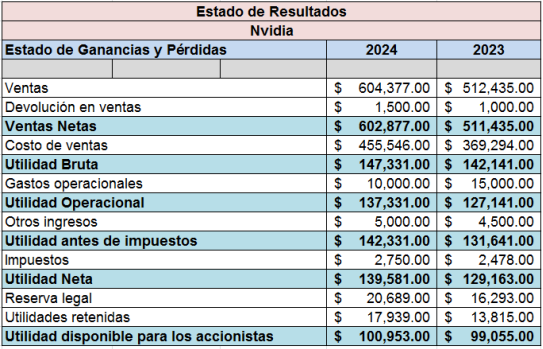
\includegraphics[width=15cm]{./assets/estado_resultados.png}
% \end{center}

\newpage

\section{Gestión del Servicio}

La gestión del servicio al cliente de Nvidia se centra en la atención al cliente, la resolución de problemas y la gestión de reclamos. La empresa se esfuerza por ofrecer una experiencia del usuario excepcional, garantizando que los clientes reciban un servicio de alta calidad que satisfaga sus necesidades y expectativas. Nvidia utiliza una combinación de estrategias para gestionar el servicio al cliente, incluyendo la formación de empleados, la implementación de procesos y procedimientos, la recopilación de feedback y la mejora continua de la calidad del servicio.
  
Algunos indicadores para una correcta gestión del servicio podemos encontrarlos aquí:

\begin{enumerate}
  \item \textbf{Tiempo de respuesta:}
  
  Mide el tiempo que tarda la empresa en responder a las consultas y solicitudes de los clientes.
  
  En ese sentido, Nvidia se esfuerza por responder a las consultas de manera automatizada por chatbots o correos electrónicos, y a las solicitudes de soporte técnico en un plazo de 24 horas.

  \item \textbf{Índice de satisfacción del cliente:}
  
  Mide la satisfacción de los clientes con el servicio recibido, a través de encuestas y feedback.
  
  Nvidia al ser una empresa en su más enfocada al modelo B2B, procura mantener su cartera de clientes satisfecha, ofreciendo soporte técnico especializado y soluciones personalizadas, de hecho, ello hace que algunos de sus productos también sean personalizados.

  \item \textbf{Índice de resolución de problemas:}
  
  Mide la eficacia de la empresa en la resolución de problemas y reclamos de los clientes.
  
  Nvidia se esfuerza por resolver los problemas y reclamos de los clientes de manera rápida y eficiente, garantizando una experiencia positiva en cada interacción. Problemas como la garantía de los productos, la devolución de los mismos, entre otros, son resueltos de manera rápida y eficiente.

  \item \textbf{Índice de fidelización de clientes:} 
  
  Mide la lealtad de los clientes hacia la empresa y sus productos, a través de la repetición de compras y recomendaciones.

  Nvidia tiene una ventaja competitiva en la fidelización de clientes, ya que sus productos son altamente especializados y de alta calidad, lo que genera una lealtad a largo plazo. Además, la empresa ofrece programas de fidelización y beneficios exclusivos para sus clientes.

  Además, Nvidia ofrece a algunos de sus clientes que adquieren productos de alta gama, accesibilidad anticipada a nuevo software basado en inteligencia artificial lo cual les permite tener una ventaja competitiva en el mercado.

  \item \textbf{Índice de calidad del servicio:}
  
  Mide la calidad del servicio ofrecido por la empresa, basado en la precisión, amabilidad y eficiencia de los empleados.

  Nvidia puede calcular este índice en comparación con la calidad de servicio de la competencia, para identificar áreas de mejora y oportunidades de diferenciación. AMD y Intel son sus competidores más cercanos, por lo que la calidad del servicio es un factor clave para mantener su posición de liderazgo en el mercado.

\end{enumerate} 
  
\newpage
\section{Gestión del Personal}

La gestión del personal de Nvidia se centra en la selección, contratación, capacitación, evaluación y desarrollo del personal. La empresa se esfuerza por atraer y retener a los mejores talentos, ofreciendo oportunidades de crecimiento y desarrollo profesional a sus empleados. La gestión del personal de Nvidia se basa en la meritocracia, la transparencia y la equidad, garantizando un ambiente de trabajo inclusivo y colaborativo.

A continuación se presenta un organigrama de la empresa Nvidia:

\begin{center}
  \begin{tikzpicture}[
    mindmap,
    grow cyclic,
    every node/.style={concept, text width=2.8cm, align=center, font=\scriptsize},
    concept color=blue!30,
    level 1/.append style={level distance=5cm, sibling angle=90},
    level 2/.append style={level distance=3.5cm, sibling angle=45},
    level 3/.append style={level distance=2.5cm, sibling angle=30}
]

% Nodo principal
\node{Director Ejecutivo\\\textbf{Jen-Hsun Huang}}
    child {node {Director Financiero\\\textbf{Colette Kress}}
        child {node {Desarrollo Corporativo\\\textbf{Vishal Bhagwati}}}
        child {node {Contabilidad\\\textbf{Donald Robertson}}}
        child {node {Impuestos\\\textbf{Michael Ching}}}
        child {node {Auditoría\\\textbf{Victoria Nguyen}}}
    }
    child {node {Científica e Investigación\\\textbf{Bill Dally}}
        child {node {Investigación\\\textbf{David Luebke}}}
        child {node {Aprendizaje Profundo\\\textbf{Bryan Catanzaro}}}
    }
    child {node {Director de Tecnología\\\textbf{Michael Kagan}}
        child {node {Telecomunicaciones\\\textbf{Ronnie Vasishta}}}
        child {node {Tecnología Avanzada\\\textbf{Joe Greco}}}
        child {node {Arquitectura de Software\\\textbf{Dror Goldenberg}}}
        child {node {Sistemas y Aplicaciones\\\textbf{Tommy Lee}}}
    }
    child {node {Operaciones\\\textbf{Debora Shoquist}}
        child {node {Gestión de Productos\\\textbf{Adel Hallak}}}
        child {node {Gestión de Productos\\\textbf{Premal Savla}}}
    };

\end{tikzpicture}

\end{center}

\newpage

\section{Selección y Retención del Personal}
 
La selección y retención del personal es un aspecto clave de la gestión del personal de Nvidia, ya que la empresa busca atraer y retener a los mejores talentos para impulsar su innovación y crecimiento.

\subsection{Sobre la selección del personal}

Nvidia utiliza una combinación de estrategias para seleccionar a los mejores talentos, incluyendo:

\begin{enumerate}
  \item Procesos de selección rigurosos: la empresa utiliza pruebas técnicas, entrevistas y evaluaciones de habilidades para evaluar a los candidatos y garantizar que cumplan con los requisitos del puesto.
  \item Evaluación de competencias: Nvidia evalúa las competencias técnicas y blandas de los candidatos, como la capacidad de resolución de problemas, la creatividad, la comunicación y la colaboración.
  \item Cultura organizacional: la empresa busca candidatos que se ajusten a su cultura organizacional, basada en la innovación, la excelencia y el trabajo en equipo.
  \item Desarrollo profesional: Nvidia ofrece oportunidades de desarrollo profesional y crecimiento a sus empleados, lo que les permite adquirir nuevas habilidades y avanzar en sus carreras.
  \item Experiencia en Investigación y Desarrollo: Nvidia valora la experiencia en investigación y desarrollo de sus empleados, ya que la innovación es un pilar fundamental de su estrategia de negocio.
\end{enumerate}

Nvidia utiliza una combinación de estrategias para seleccionar y retener a su personal, incluyendo:

\subsection{Cultura de Trabajo Positiva:}

\begin{enumerate}
  \item Ambiente inclusivo: fomenta la diversidad y la inclusión, creando un espacio de trabajo donde todos se sientan valorados y respetados. 
  \item Comunicación abierta: la empresa se esfuerza por mantener una comunicación transparente y honesta con sus empleados, informándoles sobre las estrategias, objetivos y planes de la empresa. 
  \item Trabajo en equipo: promueve la colaboración y el trabajo en equipo, creando un ambiente de apoyo y aprendizaje. 
\end{enumerate}

% DESARROLLO Y CRECIMIENTO PROFESIONAL 

% Oportunidades de aprendizaje: la empresa ofrece una variedad de cursos, talleres y programas de formación para que sus empleados puedan desarrollar nuevas habilidades y conocimientos. 

 

% Planes de carrera: define rutas de crecimiento y ascenso de manera interna, con objetivos y metas para que los empleados puedan seguir con sus carreras. 

 

% Programas de rotación: permite que sus empleados experimenten diferentes áreas y roles ampliando su experiencia y conocimiento dentro de la empresa. 

 

% RECONOCIEMINTO Y RECOMPENSAS 

% Programas de incentivos: ofrece un bono/recompensa por su desempeño, logros y contribuciones al equipo. 

 

% Beneficios competitivos: ofrece paquetes de beneficios incluyendo seguro médico, dental y de bienestar. 

 

% Reconocimiento público: celebra los logros de sus empleados y reconoce el esfuerzo e impacto en la empresa- 

 

% LIDERAZGO: 

% La empresa se enfoca en desarrollar a lideres que den soporte (apoyo) a los empleados que recién se van a integrando a la empresa para que los inspiren y motiven a seguir con su trabajo del día a día. Por ello tenemos que mantener una comunicación abierta y fluida entre los lideres y los empleados. Y así puedan desarrollar su talento nato dentro de la empresa, brindando oportunidades de crecimiento y aprendizaje. 

 

% ONBOARDING: 

% NVIDIA ofrece un programa de inducción integral para los nuevos empleados, para que introduzcan su cultura, valores y expectativas sobre el área en el que están laborando. Luego el empleado es asignado con un colaborador capacitado para que lo guie y despeje sus dudas acerca de la empresa o del puesto, además para que se incluyan con los demás, la empresa organiza actividades de integración. 

% NVIDIA, al implementar estas estrategias, crea un ambiente de trabajo atractivo y positivo que ayuda a retener a su personal. Su enfoque en el desarrollo, el reconocimiento y la cultura de trabajo les permite no solo atraer talento, sino también retenerlo a largo plazo. 


\subsection{Desarrollo y Crecimiento Profesional:}

\begin{enumerate}
  \item Oportunidades de aprendizaje: la empresa ofrece una variedad de cursos, talleres y programas de formación para que sus empleados puedan desarrollar nuevas habilidades y conocimientos.
  \item Planes de carrera: define rutas de crecimiento y ascenso de manera interna, con objetivos y metas para que los empleados puedan seguir con sus carreras.
  \item Programas de rotación: permite que sus empleados experimenten diferentes áreas y roles ampliando su experiencia y conocimiento dentro de la empresa.
\end{enumerate}

\subsection{Reconocimiento y Recompensas:}

\begin{enumerate}
  \item Programas de incentivos: ofrece un bono/recompensa por su desempeño, logros y contribuciones al equipo.
  \item Beneficios competitivos: ofrece paquetes de beneficios incluyendo seguro médico, dental y de bienestar.
  \item Reconocimiento público: celebra los logros de sus empleados y reconoce el esfuerzo e impacto en la empresa.
\end{enumerate}

\subsection{Liderazgo:}

La empresa se enfoca en desarrollar a líderes que den soporte (apoyo) a los empleados que recién se van a integrando a la empresa para que los inspiren y motiven a seguir con su trabajo del día a día. Por ello tenemos que mantener una comunicación abierta y fluida entre los líderes y los empleados. Y así puedan desarrollar su talento nato dentro de la empresa, brindando oportunidades de crecimiento y aprendizaje.

\subsection{Onboarding:}

Nvidia ofrece un programa de inducción integral para los nuevos empleados, para que introduzcan su cultura, valores y expectativas sobre el área en el que están laborando. Luego el empleado es asignado con un colaborador capacitado para que lo guie y despeje sus dudas acerca de la empresa o del puesto, además para que se incluyan con los demás, la empresa organiza actividades de integración.

Nvidia, al implementar estas estrategias, crea un ambiente de trabajo atractivo y positivo que ayuda a retener a su personal. Su enfoque en el desarrollo, el reconocimiento y la cultura de trabajo les permite no solo atraer talento, sino también retenerlo a largo plazo.

\section{Conclusiones}

En conclusión, la empresa Nvidia ha logrado establecerse como un líder en el mercado de tecnología y semiconductores gracias a su enfoque en la innovación, la calidad y la excelencia en la gestión comercial. La empresa ha demostrado una sólida estrategia de marketing mix, centrada en los pilares fundamentales de producto, precio, plaza y promoción, que le ha permitido diferenciarse y destacarse en un mercado altamente competitivo.

Además, la empresa ha demostrado una gestión de ventas efectiva, basada en la identificación de oportunidades de venta, la prospección de clientes, la presentación de propuestas comerciales, el cierre de ventas y el seguimiento postventa. Nvidia ha implementado estrategias específicas para cerrar ventas, como ofrecer valor tangible y diferenciación, paquetes de valor añadido, argumentos de rentabilidad a largo plazo, creación de escasez y exclusividad, construcción de relaciones y confianza, apoyo de socios y distribuidores, y garantías y actualizaciones.

Asimismo, la empresa ha demostrado una gestión del servicio al cliente centrada en la atención al cliente, la resolución de problemas y la gestión de reclamos. Nvidia se esfuerza por ofrecer un servicio de alta calidad que satisfaga las necesidades y expectativas de sus clientes, garantizando una experiencia positiva en cada interacción.

Finalmente, la empresa ha demostrado una gestión del personal efectiva, centrada en la selección, contratación, capacitación, evaluación y desarrollo del personal. Nvidia se esfuerza por atraer y retener a los mejores talentos, ofreciendo oportunidades de crecimiento y desarrollo profesional a sus empleados. La empresa ha implementado una serie de estrategias para seleccionar y retener a su personal, incluyendo una cultura de trabajo positiva, desarrollo y crecimiento profesional, reconocimiento y recompensas, liderazgo y onboarding.

\newpage

\begin{thebibliography}{9}

  \bibitem{paucar} 
  Paucar J. (2019) Evolución de las 4P´s o Marketing Mix. Recuperado de: \url{https://www.gestiopolis.com/evolucion-de-las-4ps-o-marketing-mix/}

  \bibitem{rojas}
  Rojas Z. (2017) La Gestión de Ventas y Rentabilidad. Recuperado de: \url{https://www.gestiopolis.com/la-gestion-ventas-la-rentabilidad/}

  \bibitem{pineiro}
  Piñeiro A. Varela J. Rail A. (2006) El análisis de importancia-valoración aplicado a la gestión de servicios. Recuperado de: \url{https://www.gestiopolis.com/el-analisis-de-importancia-valoracion-aplicado-a-la-gestion-de-servicios/}

\end{thebibliography}

  
\end{document}